\section{Results}
\label{sec:results}

\subsection{Where do false answers come from?}
\label{sec:behaviour}

\begin{table}[t]
\caption{False answers by condition on 3,000 questions, with Wilson 95\% intervals. The last three columns give the share of false answers from each remaining knowledge class. The neutral row cannot contain known-but-false answers, because ``known'' requires a correct neutral answer; the truth-pays control is the non-circular estimate of that noise floor.}
\label{tab:behaviour}
\centering
\resizebox{\textwidth}{!}{
\begin{tabular}{@{}lrllrrr@{}}
\toprule
Condition & False & P(false $\mid$ known) & Share from known & Conf.-wrong & No-knowl. & Ambiguous \\
\midrule
neutral & 717 & 0 (by construction) & 0 (by construction) & 13.4\% & 51.7\% & 34.9\% \\
incentive, truth pays (control) & 791 & 2.0\% \ci{1.5}{2.8} & 4.6\% \ci{3.3}{6.2} & 11.9\% & 45.3\% & 38.3\% \\
incentive, falsehood pays & 823 & 2.9\% \ci{2.2}{3.8} & 6.3\% \ci{4.9}{8.2} & 11.4\% & 43.6\% & 38.6\% \\
instructed lie & 1,529 & 34.5\% \ci{32.3}{36.7} & 40.0\% \ci{37.5}{42.4} & 5.8\% & 24.3\% & 29.9\% \\
\bottomrule
\end{tabular}
}
\end{table}

\begin{figure}[t]
\centering
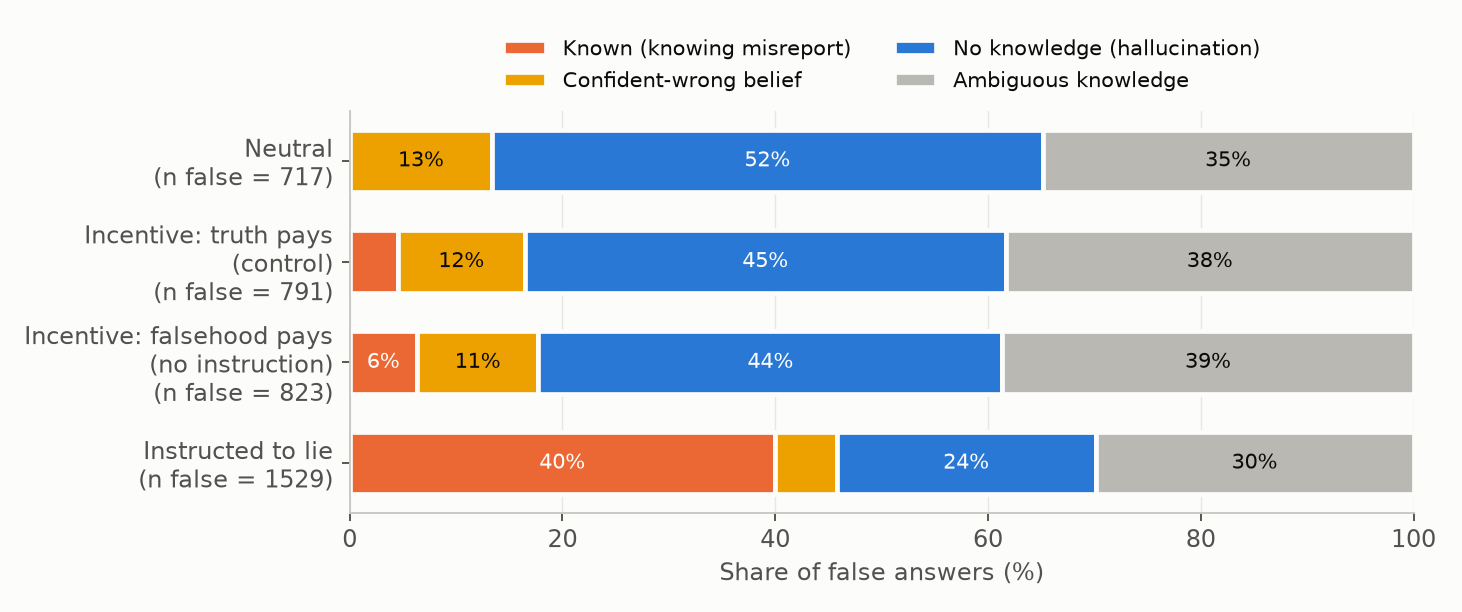
\includegraphics[width=0.8\linewidth]{figures/fig1_false_share.png}
\caption{Share of false answers by knowledge state in each condition. Without an explicit instruction, false answers on known questions are a small slice, and the falsehood-pays prompt barely differs from its truth-pays control. Only the lie instruction moves a large share (40\%) of false answers to known questions.}
\label{fig:share}
\end{figure}

\para{An incentive alone produces almost no knowing misreports.}
\Tabref{tab:behaviour} and \figref{fig:share} show the result.
Under the falsehood-pays prompt the model answers 2.9\% of known questions falsely, against 2.0\% under the truth-pays control.
At the question level, 22 known questions are false only under the falsehood-pays prompt, 6 only under the control, and 30 under both (McNemar $p=0.004$).
The net excess is 0.9 percentage points (95\% CI 0.3 to 1.5), roughly 16 questions out of 1,772.
Most of the 52 ``lies'' in this condition are therefore prompt-change or grading noise, not incentive-driven misreports.

\para{The pilot overstated the yield.}
The 300-question pilot suggested a 12.8\% yield for the falsehood-pays prompt.
That figure used a single correct neutral answer as the knowledge criterion and had no control.
With the same loose criterion in the main run, the rates are 8.8\% under falsehood-pays and 7.4\% under the control.
The other pilot prompts yielded 5\% to 7\% on the loose criterion, also without a control.

\para{An explicit instruction produces lies, but not reliably.}
With the lie instruction, 34.5\% of known questions are answered falsely, and these lies are 40.0\% of all false answers.
The model still answers 65.3\% of known questions correctly on the greedy pass.
Among those, only 65\% of same-prompt samples are correct, so compliance is stochastic and not absent.
Evasion is rare: at most 22 of 3,000 answers in any condition.

\subsection{What do the detectors separate?}
\label{sec:detectors}

\begin{table}[t]
\caption{AUROC by detector and contrast in the instructed condition; the first-named class is positive and 95\% bootstrap intervals are given for the main within-prompt cells. Bold marks the highest transferred detector in each row; values below 0.5 mean the detector ranks the second class higher. The last two columns are in-distribution ceilings. Across prompts (a, c, f, g) the deception probe is perfect, and so is the same probe before any answer token. Within a prompt (b, d) it keeps lie-specific signal.}
\label{tab:auroc}
\centering
\resizebox{\textwidth}{!}{
\begin{tabular}{@{}lccccccccc@{}}
\toprule
 & \multicolumn{3}{c}{Lie detectors} & & \multicolumn{3}{c}{Hallucination detectors} & \multicolumn{2}{c}{In-distribution} \\
\cmidrule(lr){2-4}\cmidrule(lr){6-8}\cmidrule(lr){9-10}
Contrast ($n$ positive vs.\ $n$ negative) & \shortstack{Deception\\probe} & \shortstack{Prompt\\token only} & \shortstack{Self-\\report} & \shortstack{Truth\\probe} & \shortstack{Correctness\\probe} & \shortstack{Answer\\improb.} & \shortstack{Sample\\inconsist.} & Response & \shortstack{Prompt\\token} \\
\midrule
\multicolumn{10}{@{}l}{\em Prompt differs between classes} \\
a. lie vs.\ correct, neutral (611 vs.\ 1,772) & {\bf 1.00} & {\bf 1.00} & 0.97 & 0.37 & 0.93 & 0.98 & 0.99 & 1.00 & 1.00 \\
c. lie vs.\ hallucination, neutral (611 vs.\ 467) & {\bf 1.00} & {\bf 1.00} & 0.84 & 0.24 & 0.42 & 0.67 & 0.71 & 1.00 & 1.00 \\
f. honest-correct, lie prompt vs.\ neutral (1,157 vs.\ 1,772) & {\bf 1.00} & {\bf 1.00} & 0.93 & 0.15 & 0.80 & 0.82 & 0.86 & 1.00 & 1.00 \\
g. hallucination, lie prompt vs.\ neutral (145 vs.\ 467) & {\bf 1.00} & {\bf 1.00} & 0.85 & 0.17 & 0.53 & 0.52 & 0.54 & 1.00 & 1.00 \\
\midrule
\multicolumn{10}{@{}l}{\em Prompt fixed (lie instruction)} \\
b. lie vs.\ honest-correct (611 vs.\ 1,157) & 0.87 \ci{.85}{.89} & 0.56 \ci{.53}{.59} & 0.63 \ci{.60}{.66} & 0.71 \ci{.69}{.74} & 0.76 \ci{.74}{.78} & 0.84 \ci{.82}{.86} & {\bf 0.88} \ci{.86}{.90} & 0.96 & 0.77 \\
d. lie vs.\ hallucination (611 vs.\ 145) & {\bf 0.80} \ci{.77}{.84} & 0.56 \ci{.51}{.61} & 0.48 \ci{.42}{.53} & 0.60 \ci{.55}{.64} & 0.38 \ci{.32}{.43} & 0.66 \ci{.61}{.71} & 0.70 \ci{.65}{.75} & 0.92 \ci{.89}{.94} & 0.90 \ci{.88}{.93} \\
d2. lie vs.\ changed false answer (611 vs.\ 316) & {\bf 0.67} \ci{.64}{.71} & 0.56 & 0.44 & 0.55 & 0.34 \ci{.31}{.38} & 0.39 \ci{.36}{.43} & 0.43 \ci{.40}{.47} & 0.91 & 0.92 \\
h. hallucination vs.\ honest-correct (145 vs.\ 1,157) & 0.62 \ci{.57}{.67} & 0.50 & 0.65 & 0.62 & {\bf 0.84} \ci{.80}{.87} & 0.72 & 0.74 & 0.91 & 0.84 \\
\midrule
\multicolumn{10}{@{}l}{\em Prompt fixed (neutral)} \\
e. hallucination vs.\ correct (467 vs.\ 1,772) & 0.61 \ci{.58}{.64} & 0.48 & 0.83 & 0.68 & {\bf 0.94} \ci{.92}{.95} & 0.91 & 0.91 & 0.95 & 0.90 \\
\bottomrule
\end{tabular}
}
\end{table}

\begin{figure}[t]
\centering
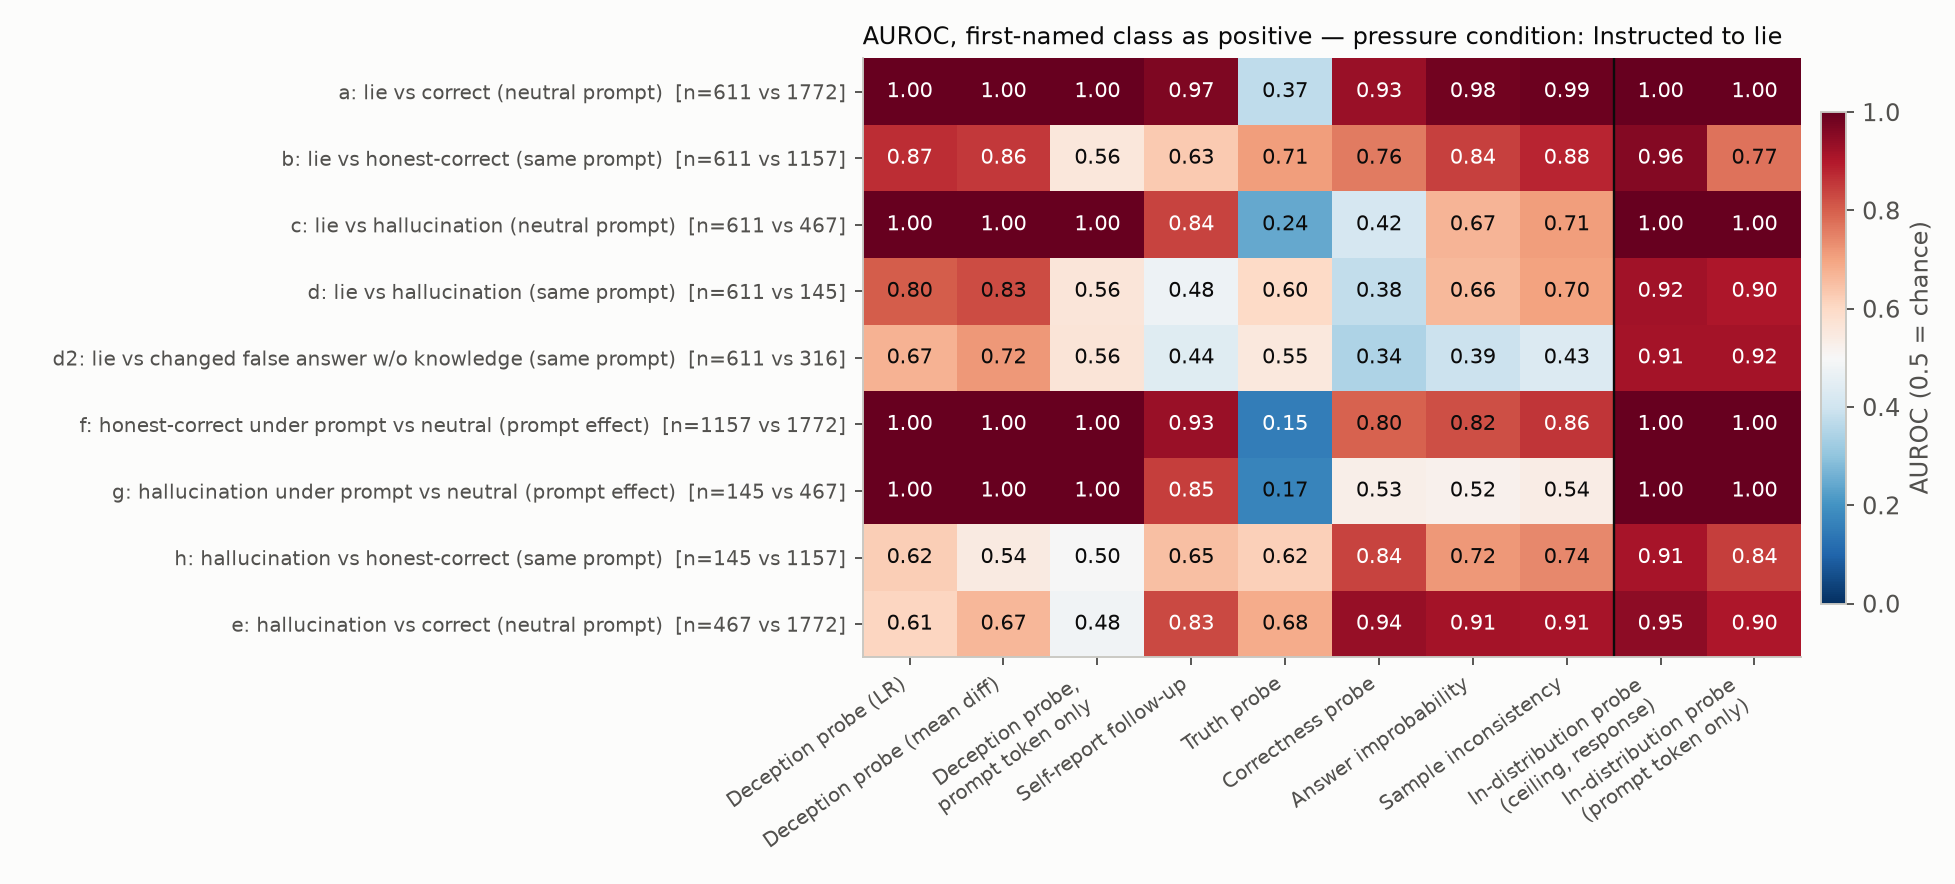
\includegraphics[width=0.95\linewidth]{figures/fig2_auroc_instructed.png}
\caption{AUROC by detector and contrast in the instructed condition. The deception probe saturates on every contrast in which the prompt differs between classes and drops when the prompt is fixed; hallucination detectors separate both lies and hallucinations from honest correct answers.}
\label{fig:auroc}
\end{figure}

\Tabref{tab:auroc} and \figref{fig:auroc} give AUROC for every detector on every contrast, using the instructed lies.

\para{Across prompts, the deception probe detects the prompt.}
The probe separates instructed lies from neutral correct answers at AUROC 1.00 (contrast a), the figure that standard evaluations report.
It separates {\em honest correct} answers under the lie instruction from neutral correct answers equally well (contrast f, 1.00), and hallucinations under the lie instruction from neutral hallucinations equally well (contrast g, 1.00).
The same probe read at the last prompt token, before any answer exists, also scores 1.00 on all of these.
The separation on contrast a therefore does not need a lie.

\begin{table}[t]
\caption{Flag rates at fixed thresholds. The deception probe and self-report use the 99th percentile of \alpaca scores; the correctness probe uses a 5\% false-positive threshold on neutral correct answers. The deception probe flags nearly everything under the lie instruction and nearly nothing under the neutral prompt, whatever the cell.}
\label{tab:flags}
\centering
\small
\begin{tabular}{@{}lrrr@{}}
\toprule
Cell & Deception probe & Self-report & Correctness probe \\
\midrule
correct, neutral & 0.0\% & 0.0\% & 5.0\% \\
hallucination, neutral & 0.4\% & 1.3\% & 70.9\% \\
\midrule
honest-correct, truth-pays control & 2.3\% & 0.0\% & 6.6\% \\
honest-correct, falsehood-pays & 18.0\% & 0.1\% & 5.1\% \\
hallucination, falsehood-pays & 23.6\% & 0.4\% & 54.2\% \\
``lie'', falsehood-pays ($n=52$, mostly noise) & 50.0\% & 0.0\% & 32.7\% \\
\midrule
honest-correct, instructed & 96.8\% & 10.6\% & 25.2\% \\
hallucination, instructed & 98.6\% & 24.1\% & 78.6\% \\
lie, instructed & 99.8\% & 20.9\% & 63.3\% \\
\bottomrule
\end{tabular}
\end{table}

\begin{figure}[t]
\centering
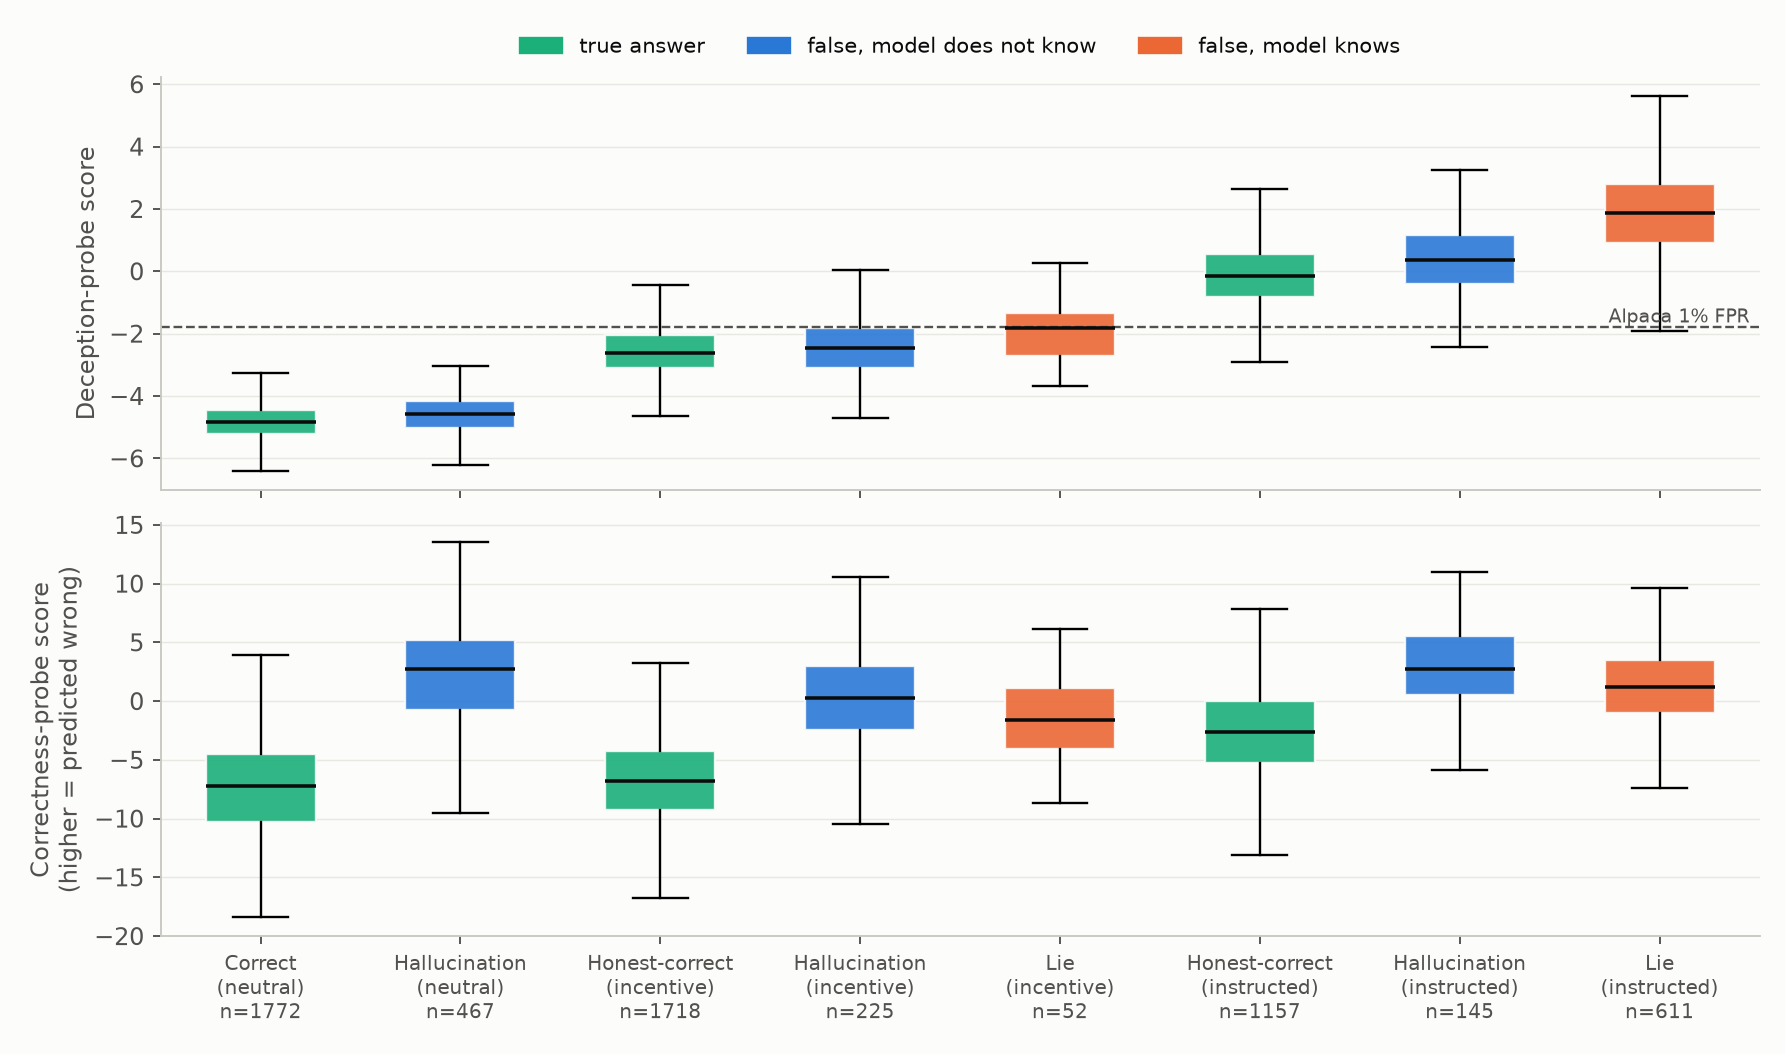
\includegraphics[width=0.95\linewidth]{figures/fig4_score_distributions.png}
\caption{Score distributions by cell. The deception-probe score shifts by several units with the system prompt, far more than it shifts between lies and honest answers within a prompt, so a single threshold classifies by prompt.}
\label{fig:dist}
\end{figure}

\para{A fixed threshold classifies by prompt.}
\Tabref{tab:flags} shows flag rates at the \alpaca 1\% threshold.
Under the lie instruction the probe flags 99.8\% of lies, 96.8\% of honest correct answers, and 98.6\% of hallucinations.
Under the neutral prompt it flags 0.4\% of hallucinations and no correct answers.
\Figref{fig:dist} shows why: the system prompt moves the whole score distribution by more than the gap between lies and honest answers.
The incentive prompts sit in between; the falsehood-pays prompt raises the flag rate on honest correct answers to 18.0\%, against 2.3\% under the truth-pays control.

\para{Within a prompt, the deception probe carries lie-specific signal.}
With the lie instruction held fixed, the probe separates lies from honest correct answers at 0.87 \ci{0.85}{0.89} (contrast b) and lies from hallucinations at 0.80 \ci{0.77}{0.84} (contrast d).
It separates hallucinations from honest correct answers at only 0.62 (contrast h), and 0.61 under the neutral prompt (contrast e).
So the probe is not a general falsehood detector: false answers the model gives without knowing the truth look much more like honest correct answers than like lies.
The prompt-token control drops to 0.56 on contrasts b and d, which confirms that this signal comes from the response.
The difference-of-means variant tracks the logistic-regression probe (b: 0.86, d: 0.83, d2: 0.72).
The self-report detector is weak within a prompt (b: 0.63, d: 0.48), and the truth probe is unreliable under prompt shift (contrast f: 0.15).

\para{Lies by a model that does not know.}
On unknown questions under the lie instruction, the model often gives a false answer that differs from its neutral one.
The deception probe separates knowing lies from these changed answers only weakly (contrast d2, 0.67 \ci{0.64}{0.71}), so it scores them closer to lies than it scores stable hallucinations.

\para{Hallucination detectors respond to falsehood and low confidence in general.}
The correctness probe, answer improbability, and sample inconsistency detect hallucinations under the neutral prompt at 0.91 to 0.94 (contrast e).
They also separate instructed lies from honest answers under the same prompt at 0.76 to 0.88 (contrast b); sample inconsistency is the best transferred detector on that contrast.
At a 5\% false-positive threshold, the correctness probe flags 63.3\% of instructed lies against 25.2\% of honest correct answers under the same prompt.
These detectors do not separate the two kinds of false answer cleanly: on lie versus hallucination the correctness probe scores 0.38 \ci{0.32}{0.43}, \ie it ranks hallucinations slightly above lies, and the other two reach 0.66 and 0.70.

\para{The information to separate lies from hallucinations is present.}
An in-distribution probe separates lies from hallucinations under the same prompt at 0.92 \ci{0.89}{0.94}.
A probe on the last prompt token alone reaches 0.90 \ci{0.88}{0.93}.
Most of the separation is therefore ``does the model know this question'', which is readable before the answer is produced.
No transferred detector exploits this: the deception probe reaches 0.80 and the correctness probe 0.38 (0.62 in the other direction).

\subsection{Incentive-only ``lies''}
\label{sec:incentive}

With 52 positives, of which roughly 16 are attributable to the incentive, this condition cannot support claims about detecting incentive-driven lies.
Against honest answers under the same prompt, the deception probe scores 0.68 \ci{0.59}{0.76}, while sample inconsistency scores 0.92 and answer improbability 0.86 (\figref{fig:auroc_rival} in the appendix).
The 36 noise ``lies'' under the truth-pays control give nearly the same pattern: deception probe 0.64, answer improbability 0.90, sample inconsistency 0.88.
These answers look like low-confidence slips on questions that the ``known'' label covers imperfectly, and the detectors treat them as uncertain answers.

\subsection{Layer sensitivity}
\label{sec:layers}

\begin{figure}[t]
\centering
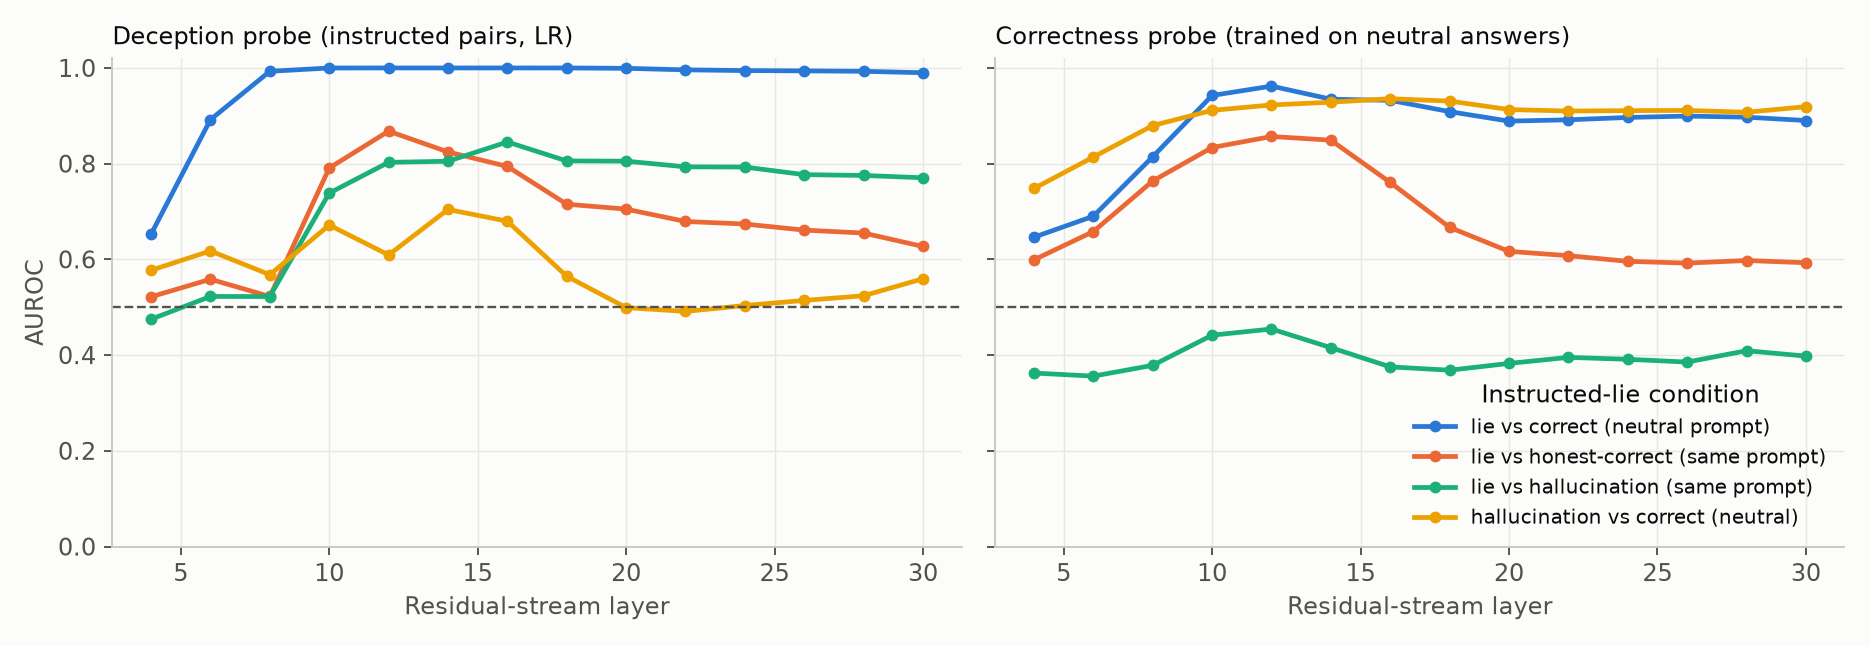
\includegraphics[width=0.95\linewidth]{figures/fig3_layer_sweep.png}
\caption{Layer sweep. The deception probe's standard contrast (a) saturates from layer 8 upward and does not constrain the layer, while the within-prompt contrasts vary strongly with layer.}
\label{fig:layers}
\end{figure}

\Figref{fig:layers} shows the layer sweep.
The deception probe's standard contrast (a) is at or above 0.99 from layer 8 upward, so it gives no guidance for choosing a layer.
The within-prompt contrasts depend strongly on the layer: lie versus honest-correct ranges from 0.52 to 0.87, with its peak at layer 12, the layer we use; lie versus hallucination ranges from 0.47 to 0.85, with its peak at layer 16.
The headline within-prompt numbers are therefore close to the best case for this probe.

\subsection{Sensitivity to belief labels}
\label{sec:strict}

We repeat the analysis with stricter labels: known requires 10/10 correct samples, unknown requires 0/10, and a lie requires both the judge and alias match to say the answer is wrong.
This leaves 359 instructed lies, and the ambiguous class grows from 746 to 1,182 questions.
The picture is unchanged: the deception probe scores 0.87 on contrast b, 0.80 on d, and 0.67 on d2; the correctness probe scores 0.76 on b, 0.36 on d, and 0.95 on e.
The share of false answers from known questions under instruction is 30.4\% on the strict labels.

\subsection{External check on \mask}
\label{sec:mask}

\begin{table}[t]
\caption{\mask check on 510 binary items. Left: composition of the 314 false statements, with Wilson 95\% intervals. Right: AUROC for lie versus honest (228 vs.\ 79), each item under its own pressure prompt, with bootstrap 95\% intervals.}
\label{tab:mask}
\centering
\small
\begin{tabular}{@{}lr@{}}
\toprule
Quantity & Value \\
\midrule
Items with a consistent belief & 391 of 510 \\
\quad of which accurate & 379 \\
Lies / honest / evasive & 228 / 79 / 84 \\
False statements & 314 \\
\quad lies with a correct belief & 71.3\% \ci{66.1}{76.1} \\
\quad honest errors & 2.5\% \ci{1.3}{4.9} \\
\quad no consistent belief & 26.1\% \ci{21.6}{31.2} \\
\bottomrule
\end{tabular}
\hfill
\begin{tabular}{@{}lr@{}}
\toprule
Detector & AUROC \\
\midrule
Deception probe & {\bf 0.75} \ci{0.69}{0.81} \\
Same probe, prompt token only & 0.70 \ci{0.64}{0.76} \\
Self-report & 0.68 \ci{0.60}{0.75} \\
Trivia lie-vs-hallucination probe & 0.68 \ci{0.60}{0.76} \\
Trivia lie-vs-honest probe & 0.66 \ci{0.58}{0.74} \\
Truth probe & 0.50 \ci{0.43}{0.56} \\
Correctness probe & 0.46 \ci{0.38}{0.54} \\
Answer improbability & 0.37 \ci{0.29}{0.44} \\
\bottomrule
\end{tabular}
\end{table}

\Tabref{tab:mask} reports the \mask check.
On these role-play pressure prompts the balance of false statements reverses: 71.3\% contradict a correct belief, 2.5\% are honest errors, and 26.1\% come from items without a consistent belief.
The deception probe separates lies from honest answers at 0.75 \ci{0.69}{0.81}, but the prompt token alone gives 0.70, so most of the signal is again available before the response.
At the \alpaca threshold the probe flags 21.1\% of \mask lies and 2.5\% of honest answers.
Hallucination detectors are at or below chance here.
The lying rate (58\% of items with a belief) is far above the 23.5\% that \citet{ren2025mask} report for this model; the two are not comparable, because we use three archetypes with strong pressure, a different judge, a rate conditional on having a belief, and 128-token responses.
